%!TEX root = ../paper.tex
\section{Video Classification in Caffe}
\label{sec:classification}

For building our artificial neural network we used the framework Caffe\footnote{\url{http://caffe.berkeleyvision.org/}}.
Caffe is a deep learning framework offering several implementations of layers.
Besides, Caffe is GitHub project and can be adapted and extended for special use cases.
We used with the Caffe branch of Jeff Donahue\footnote{\url{https://github.com/BVLC/caffe/pull/2033}}, which offers an implementation for long-short-term memory (LSTM).

The architecture of our artificial neural network was build on the work of TODO.
This architecture consists of three parts and can be found in Figure~\ref{fig:architecture}.
The first part is processing the single frames of a video, further called \emph{spatial}.
It is responsible for recognizing objects and structures in frames.
The second part memorizes motion of actions.
It handles flow images and is therefore called \emph{flow}.
Both parts consists of a convolutional neural network (CNN) followed by a long-short-term memory (LSTM).
To merge the predictions of both parts, \emph{spatial} and \emph{flow}, a third part is introduced.
This part, called \emph{fusion}, takes the output of both CNNs, \emph{spatial} and \emph{flow}, and merge the predictions.
To get a final overall prediction the three results are combined in the end.

\begin{figure}[!htb]
	\centering
	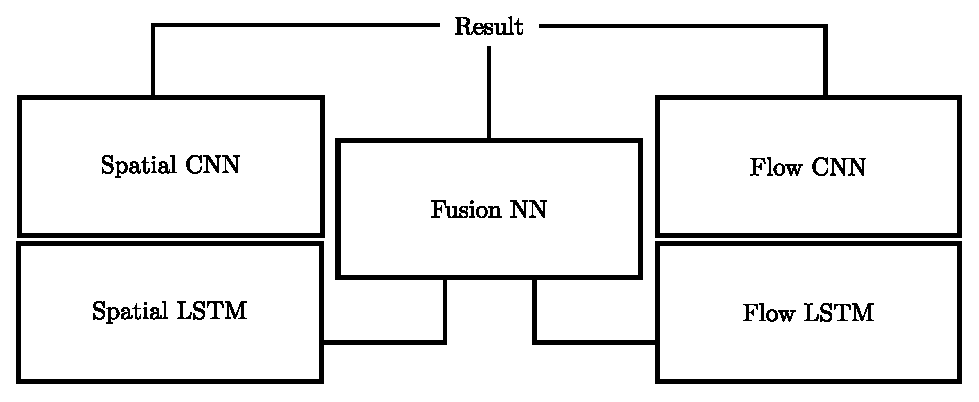
\includegraphics[scale=.7]{images/architecture.eps}
	\caption{General Architecture TODO}
	\label{fig:architecture}
\end{figure}

The individual neural networks we used in this architecture differ from the work of TODO.
Also we adapt the architecture by removing the LSTMs, only having a CNN for the \emph{spatial} and \emph{flow} part.
This is because our results using LSTMs were no that good as using only CNNs.\todo{Correct?}
During our research we tried out different neural networks, which will be presented in this section.
Also the parameters, which were used for the training, and the results will be shown.

\subsection{Changes to Caffe}

Working with a neural network consisting of LSTMs requires to use two different inputs:
On the one hand the raw pixel values and on the other hand a tagging sequence.
The tagging sequence tells the LSTM, where a new training example starts.
This is important, as there is more than one training sequence per batch.
A tagging sequence consist of 0's and 1's.
A 1 indicates the beginning of a new sequence.
For generating this tagging sequence we wrote a new data-generation strategy for the \emph{DummyData} layer.
This layer can be used for generating artifical data: Existing implementations generate constant, uniformly distributed, gaussian distributed data etc.
An example of the dummy data layer can be found in Listing~\ref{lst:seq-layer}.
The layer has the two parameters:
The first parameter is the \texttt{shape}.
The shape parameter tells the output shape of the tagging blob, i.e. \texttt{16 x 4} in the example.
The second parameter \texttt{data\_filler} tells the concrete parameters for the dummy data.
In our case, we specify the tagging sequence data generation type.
The parameter \texttt{value} specifies the length of a sequence.
In the example, this means that there is 1 one, and then 15 following zeroes.

\begin{lstlisting}[language=sh, caption=Sequence Layer, label=lst:seq-layer]
layer {
	name: "sequence"
	type: "DummyData"
	top: "sequence"
	dummy_data_param {
		shape {
			dim: 16
			dim: 4
		}
		data_filler {
			type: "sequence"
			value: 16
		}
	}
}
\end{lstlisting}

A second adaption we made to Caffe was the implementation of the script \emph{convert\_imageset\_multi}, which was already introduced in Section~\ref{sec:data}.

% \begin{itemize}
% 	\item New sequence data layer
% 	\item Multi-layer script
% 	\item More?
% \end{itemize}

\subsection{Experiment infrastructure}
For running experiments with different parameter settings, we build a script, which helps with keeping track of different experiments.
It can be found in the \texttt{nets/*} subfolders under the name \texttt{train.sh}.
It is started like \texttt{train.sh dropout0.7fps30}, where the parameter indicates the name of the experiment.
This automatically creates a folder \texttt{experiments/20150907-100235_dropout0.7fps30}, where the first numbers indicate the date and time of the experiment.
Before starting the experiment in Caffe, the script automatically copies the net and solver definitions to this folder.
After the training has finished or has been aborted, it copies the logs and the latest snapshots to the same folder.
It also automatically parses the logs and creates charts, which plot the iteration number against training loss, learning rate and test accuracy.
We used this script for all of our experiments and think it is of great value.

\subsection{Spatial}
\label{subsec:spatial}

\begin{itemize}
	\item
		Different nets:
		\begin{itemize}
			\item Caffenet/CNN\_M (also tried, VGG 19, but too big)
			\item With weights/without weights
			\item Compare the nets with respect to memory, number of parameters, training time, performance
		\end{itemize}
	\item
		Experiments:
		\begin{itemize}
			\item Different dropouts
			\item Train from scratch vs train from weights
			\item On different splits?
			\item Fc6, Fc7, fc8
			\item Different base data sets (only 16, all data)
			\item Different flows?
			\item Occlusion tests
		\end{itemize}
	\item
		LSTM did not work out
\end{itemize}


\subsection{Flow}
\label{subsec:flow}



\subsection{Fusion}
\label{subsec:fusion}

To combine the results from \emph{spatial} and \emph{flow} we use a third fusion network.
We tried out different approaches which are presented in the following.

\subsubsection{SVM}

\subsubsection{Early Fusion}
Our \emph{early fusion} architecture was build on the fusion architecture presented by TODO.
We took the CNN\_Ms for \emph{spatial} and \emph{flow} presented above and build a fusion architecture on top of them.
We selected 16 frames per video as described in Section~\ref{sec:data} and pass them on to the CNNs for \emph{spatial} and \emph{flow}.
The CNNs were cut off after the \textit{fc6}-layer having an output of 1 x 4096 per frame.
Having 16 frames in total this corresponds to an input of 16 x 4096 for both \emph{spatial} and \emph{flow} for the fusion net.
The first step in the fusion network is to merge the 16 predictions of one video into one prediction of the whole video for both \emph{spatial} and \emph{flow}.
This is done by taking the average prediction.
A fully-connected layer is then trained with those predictions before we concatenate the predictions of \emph{spatial} and \emph{flow}.
In the end two fully-connected layer are trained on the merged predictions.
The output is defined by an accuracy layer.
The whole architecture is shown in Figure~\ref{fig:early_fusion}.
\begin{figure}[!htb]
	\centering
	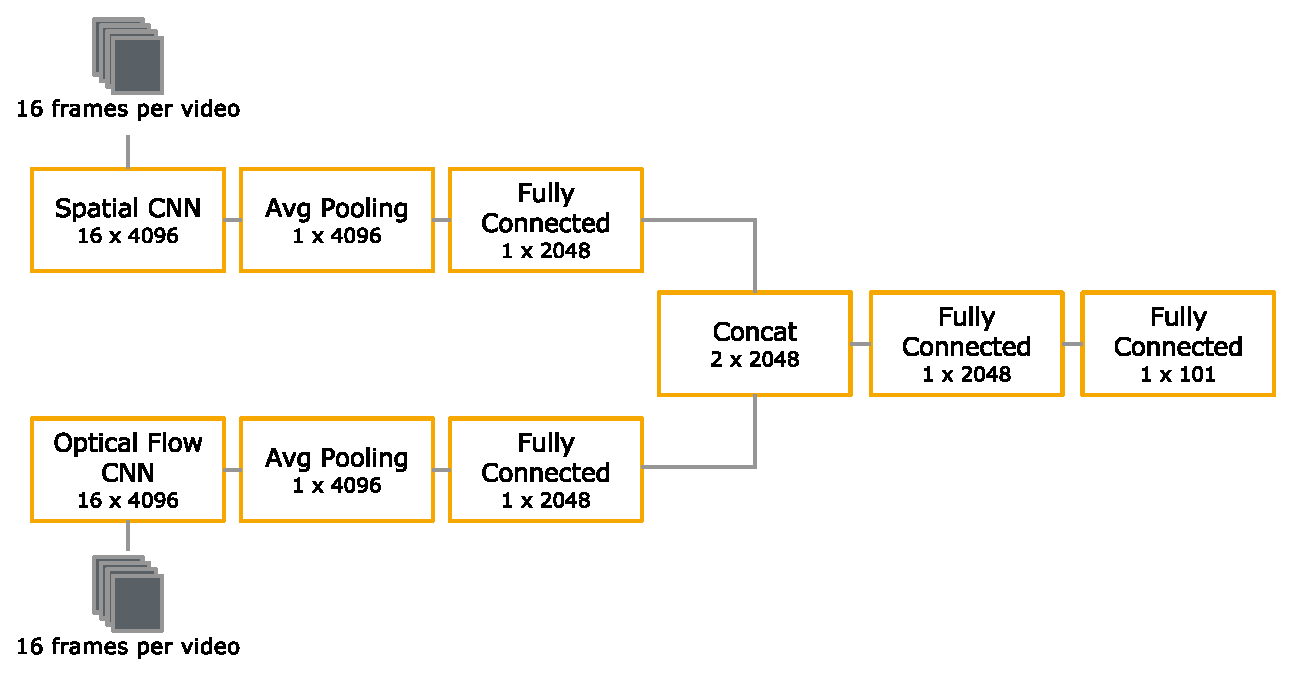
\includegraphics[scale=.7]{images/early_fusion.eps}
	\caption{Early fusion architecture: The predictions per frame of one video from the spatial and flow net are merged into one prediction per video each. Those predictions are then merged and trained via two fully connected layers.}
	\label{fig:early_fusion}
\end{figure}

TODO: results and parameter we tried

\subsubsection{Middle Fusion}


\subsubsection{Late Fusion}


\begin{figure}[!htb]
	\centering
	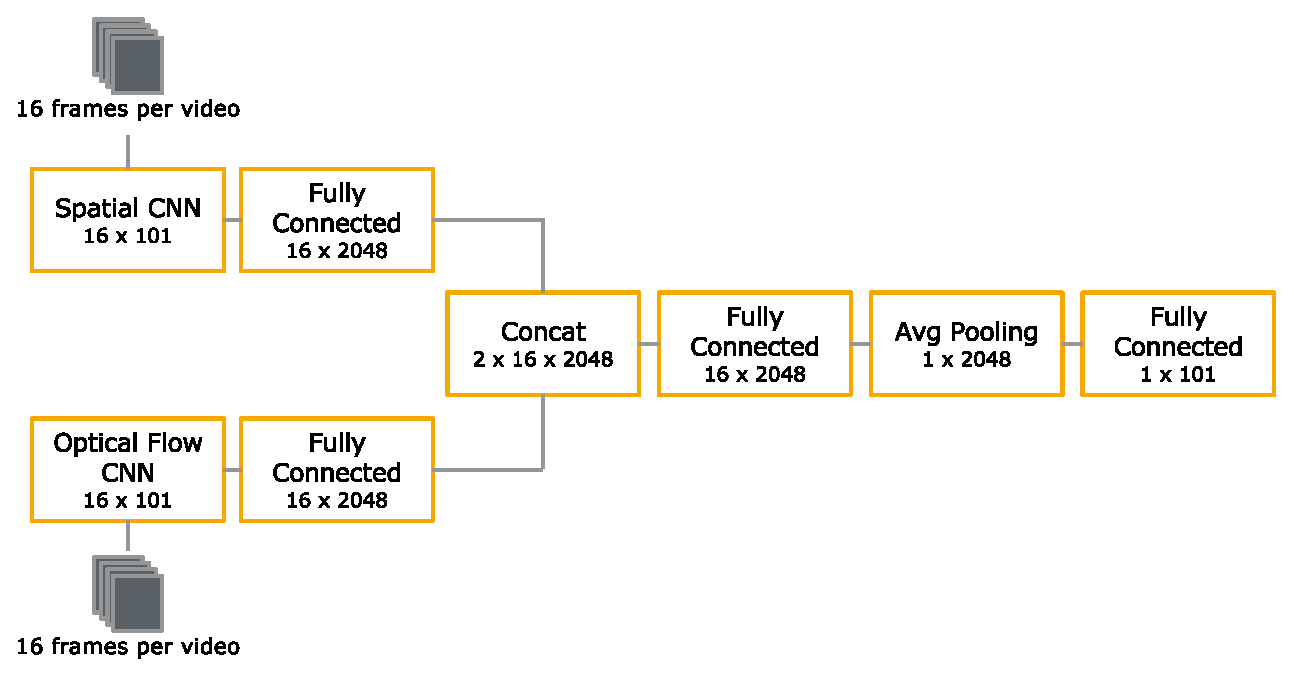
\includegraphics[scale=.7]{images/late_fusion.eps}
	\caption{}
	\label{fig:late_fusion}
\end{figure}



